\documentclass{standalone}
 
% Required package
\usepackage{tikz}
\usepackage{amssymb}
\usepackage{ntheorem}
\usepackage{tensor}
%\usepackage{physics}
\usepackage[italicdiff]{physics}
\usepackage{calc}
\usepackage{mathrsfs}
 \usetikzlibrary {backgrounds,mindmap}
 \usetikzlibrary{decorations.pathmorphing,decorations.markings}
\usetikzlibrary{decorations.pathreplacing} %
\begin{document}
 
\begin{tikzpicture}[
    mindmap,
    concept color = gray!30,
    every node/.style = {concept},
    grow cyclic,
    minimum size=5cm,
    every annotation/.style={fill=gray!3},
    level 1/.append style = {
        concept color = gray!30,
        minimum size=4cm,
        level distance = 4.5cm,
        sibling angle = 120
    },
    level 2/.append style = {
        concept color = gray!30,
        minimum size=3.5cm,
        level distance = 3cm,
        sibling angle = 45
    },
    level 3/.append style = {
        concept color = gray!30,
        minimum size=3.5cm,
        level distance = 3cm,
        sibling angle = 45
    }
]
\tikzstyle{circle connection bar}=[to path={
  [every circle connection bar]
  decorate [decoration={snake}]
  { -- (\tikztotarget) \tikztonodes}
},
append after command={[fill=olive,draw=olive]}
]

\tikzstyle{example}=[{circle,decoration=saw,decorate,fill=gray!10,inner sep=8pt}]
\definecolor{def}{RGB}{240,230,230}
 
\coordinate(N1) at (-13.5,73) {} {} {} {} {} {} {} ;
\coordinate(N2) at (10,73) {} {} {} {} {} {};
\coordinate(N3) at (-0.5,58.5) {} {} {} {} {} {} {} {} {} ;
\coordinate(N4) at (-14.5,49) {} {} {} {} {} {} {} {} {} {};
\coordinate(N5) at (9.5,65) {} {} {};
\coordinate(N6) at (9.5,55) {} {} {} {};
\coordinate(N7) at (-15,43.5) {} {} {} {} {} {} ;
\coordinate(N8) at (-19.5,33) {} {} {} {} ;
\coordinate(N9) at (-3,7) {} {} {} {} ;
\coordinate(N10) at (-23,19) {} {} {} {} ;
\coordinate(N11) at (-16.5,19) {} {} {} {} {} {} {} {} {} {} ;
\coordinate(N12) at (-3,20) {} {} {} {} {} ;
\coordinate(N13) at (-23,7) {} {} {} {} {} ;
\coordinate(N14) at (-6,30.5) {} {} {} {} {} {};
\coordinate(N15) at (2.5,48) {} {} {} {} {} {} {};
\coordinate(N16) at (-37.5,42) {} {} {};
\coordinate(N17) at (-13,23.5) {} {} {} {} {} {} {};
\coordinate(N18) at (-33.5,74) {} {} {} {} {} {} {} {};
\coordinate(N19) at (-45,55.5) {};
\coordinate(N20) at (-1.5,50) {} {};




%Inner product
\node (IP) [concept,minimum size=6cm]
 at (N1){Inner product $$<u,v>:V\times V\rightarrow \mathbb{F}$$ }
child [grow = north west]{node[left,fill=def](IP4)  { Dot product  $x,y \in \mathbb{R}^n : x.y = x_1y_1+\dots +x_ny_n$}
}
child [grow = north east]{node[minimum size=3.2cm,right,fill=def](IP5)  { Norm $$\left\| v\right\|=\sqrt{<v,v>}$$}
};
\node [annotation,below,text width = 6cm,fill=def] at (IP.south){\textbf{Positivity}\newline \newline$<v,v>\ge 0,\forall v\in V$\newline\newline

\textbf{Definiteness}\newline $<v,v>=0\Leftrightarrow v=0$\newline\newline

\textbf{Additive in the first slot}\newline \newline$<u+v,w>= <u,w>+<v,w>,\  \forall u,v,w \in V$\newline\newline

\textbf{Homogeneous in first slot}\newline\newline $<\lambda u,v>= \lambda <u,v>,\ \forall \lambda \in \mathbb{F}, \forall u,v\in V$\newline\newline

\textbf{Conjugate Symmetry}\newline\newline $<u,v>= \overline {<v,u>},\ \forall u, v\in V$\newline\newline
};
\node [annotation,left,fill = def] at (IP.west){\textbf{Inner product Space}\newline\newline
An inner product space is a vector space $V$ equipped with an innner product on $V$.};
\node [annotation,right,text width = 6.9cm] at (IP.east){\textbf{Properties}\newline\newline
$\begin{array}{ll}
\bullet& \forall \ fixed u \in V:\ <v,u> \text{ is a linear map from }V \ to \mathbb{F}\\\\
\bullet& <0,u> = 0,\ \forall u \in V\\\\
\bullet &<u,0> = 0,\ \forall u \in V\\\\
\bullet& <u,v+w> = <u,v>+ <u,w> \ \forall u,v \in V\\\\
\bullet& <u,\lambda v> = \overline{\lambda}<u,v>, \ \forall \lambda \ in \mathbb{F} \ and\ u,v\in V
\end{array}$
};
\node [annotation,right] at (IP5.east){$\bullet\quad \left\| v\right\|=0\Leftrightarrow \ v=0$\newline\newline
$\bullet\quad \left\| \lambda v\right\| = |\lambda|\left\| v\right\|,\  \forall \lambda \in\mathbb{F}$};

%Orthogonal
\node (Orth) [concept,minimum size=6cm]
 at (N2){Orthogonality$$u,v\in V: <u,v>=0$$ }
;
\node [annotation,left,text width = 6cm] at (Orth.west){Orthogonality and 0\newline\newline
$\bullet\quad 0$ is orthogonal to every vector in $V$\newline\newline
$\bullet\quad 0$ is the only vector in $V$ that is orhogonal to itself.};
\node [annotation,right] at (Orth.south east){Pythogorean Theorem\newline\newline
If $u,v\in V$ are orthogonal vectors, then,\newline\newline
$\left\| u+v\right\|^2 = \left\| u\right\|^2+\left\| v\right\|^2$};

\node [annotation,above, text width=5cm ] at (Orth.north){Orthogonal decomposition\newline\newline
Be $u,v\in V:\ v\ne 0$\newline\newline
then,\newline\newline
Set $c=\frac{<u,v>}{\left\| v\right\|^2}$ and $w= u- \frac{<u,v>}{\left\| v\right\|^2}v$\newline\newline
$<w,v>=0$ and $u=cv+w$};

\node [annotation,right, text width=5cm ] at (Orth.east){Cauchy-Schwarz Inequality \newline\newline
Be $u,v\in V$, Then,\newline\newline
$|<u,v>| \le \left\| u\right\|\left\| v \right\|$};

\node [annotation,below, text width=5cm ] at (Orth.south){\textbf{Triangle Inequality}\newline\newline
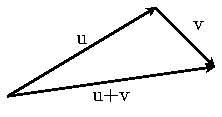
\includegraphics[width=2cm]{fig173.pdf}\newline\newline
Be $u,v\in V:\ v\ne 0$
then,\newline\newline
 $\left\| u+v\right\|\le  \left\| u \right\| +\left\| v \right\|$\newline\newline
 \textbf{Parallelogram Equality}\newline\newline
 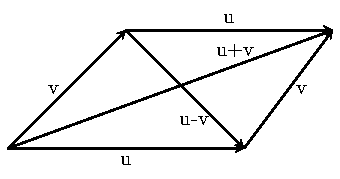
\includegraphics[width=2cm]{fig174.pdf}\newline\newline
Be $u,v\in V:\ v\ne 0$\newline\newline
then,\newline\newline
 $\left\| u+v\right\|^2 + \left\| u-v\right\|^2=  2\left(\left\| u \right\|^2 +\left\| v \right\|^2\right)$};


%Orthonormal bases
\node (OB) [concept,minimum size=6.5cm]
 at (N3){Orthonormal bases $$e_1\dots e_m \in V$$ is orthonormal if
$$  <e_j,e_k> = \left\{\begin{array}{ll} 1 & j= k\\\\
0& j\neq k\end{array}\right.$$ };
\node [annotation,below,text width = 5.5cm,] at (OB.south){Be $e_1\dots e_m$ an orthonormal list in $V$\newline\newline
$\left\| a_1e_1+\dots + a_me_m\right\|^2= |a_1|^2+\dots |a_m|^2$\newline \newline $\forall a_1\dots a_m \in \mathbb{F} $};
\node [annotation,left,fill = def] at (OB.west){\textbf{Orthonormal basis of $V$}\newline\newline
is an orthonormal list of vectors of $V$ that is also a basis of $V$.};
\node [annotation,right,text width = 4cm] at (OB.east){\textbf{Orthonormal list is linearly independent.}
\newline\newline \textbf{Orthonormal list of length $dim\ V$ is an orthonormal basis of $V$}
};




%Applications of Orthonormal bases, 
\node (AOB) [,text width = 3.5cm,concept, fill = gray!5]
 at (N4){Applications of Orthonormal bases,}
 child [grow = north ]{node[minimum size=3.2cm,above,fill= gray!5](AOB1)  { Upper-triangular matrix}
};
\node [annotation,below,text width = 5.5cm,] at (AOB.south){Be $e_1\dots e_m$ an orthonormal list in $V$\newline\newline
and $V\in V$, then\newline\newline
$v=<v,e_1>e_1+\dots + <v,e_n>e_n$\newline \newline and\newline\newline
$\left\|v\right\|^2= |<v,e_1>|^2+\dots + |<v,e_n>|^2$};
\node [annotation,right,text width = 5.5cm] at (AOB.east){\textbf{Gram-Schmidt Procedure}\newline\newline
Be $v_1,\dots,v_m$ linearly independent $\in V$\newline\newline
Let $ e_1= \frac{v_1}{\left\|v_1\right\|}$\newline\newline
For $j=2,\dots,m$ define $e_j$ inductively by \newline\newline
$ e_j= \frac{v_j -<v_j,e_1>e_1-\dots - <v_j,e_{j-1}>e_{j-1}}{\left\| v_j -<v_j,e_1>e_1-\dots - <v_j,e_{j-1}>e_{j-1}\right\| }$
};
\node [annotation,left,text width = 5.5cm,] at (AOB.west){$\bullet$ Every finite-dimensional inner product space has an orthonormal basis.\newline\newline
$\bullet$ Be $V$ finite-dimensional. Then , every orthonormal list of vectors  $\in V$ can be extended to an orthonormal basis of $V$.};

\node [annotation,left,text width = 5.5cm,] at (AOB1.west){Be $T\in \mathscr{L}\left(V\right)$. If $T$ has an upper-triangular matrix with respect to some basis of $ V$. Then,\newline\newline
$T$ has an upper-triangular matrix with respect to some orthonormal basis of $V$.};

\node [annotation,above,text width = 5.5cm,] at (AOB1.north){\textbf{Schur's Theorem}\newline\newline
Be $V$ a finite-dimensional \textbf{complex}  vector space and $T\in \mathscr{L}\left(V\right)$. Then, \newline\newline
$T$ has an upper-trianguler matrix with respect to some orthonormal basis of $V$.};

\node [annotation,right,text width = 5.5cm] at (AOB1.east){\textbf{Riezz Representation Theorem}\newline\newline
Be $V$ a finite-dimensional vector space and $\phi$ a linear functional on $V$. Then, \newline\newline
there is a unique vector $u\in V$ such that \newline\newline
$\phi(v)= <v,u>,\quad \forall v\in V.$};

\begin{pgfonlayer}{background}
\draw [concept connection, ]  (IP) edge (Orth);
\draw [concept connection, ]  (OB) edge (Orth);
\draw [concept connection, ]  (OB) edge (IP);
\draw [concept connection, ]  (AOB) edge (OB);
  \end{pgfonlayer}
\end{tikzpicture}
 
\end{document}